\chapter{Bewertung verschiedener Methoden}

Nachfolgend werden die verschiedenen Arten von CAPTCHA sowie einige Alternativen, wie Honeypots, Anti-Spam-Plugins, 
Multi-Faktor-Authentifikation und biometrische Verfahren auf Basis der zuvor entwickelten Matrix bewertet. 
Dafür wird sich an den in Kapitel \ref{ch:matrix} aufgestellten Leitfragen soweit möglich orientiert.

\section{Textbasierte CAPTCHA}
Durch ihren simplen Aufbau sind textbasierte CAPTCHAs relativ einfach zu verstehen.
Es sind wenige Clicks nötig, um einen solchen CAPTCHA auszufüllen. 
Bei optisch verzerrten Wörtern besteht jedoch die Möglichkeit, dass es zu Missverständnissen kommen kann.
So können beispielsweise ein kleines ``d'' und ein ``cl'' unter Umständen auch von Menschen verwechselt werden. 
In \autoref{fig:schwierig} ist ein ähnlicher Fall dargestellt. 
Wenn man sich nicht bewusst ist, dass hier nur korrekte Wörter der englischen Sprache erfragt werden,
kann das zweite Wort (``blotch'') auch als ``bbtch'' interpretiert werden.

\begin{figure}[h!]
    \centering
    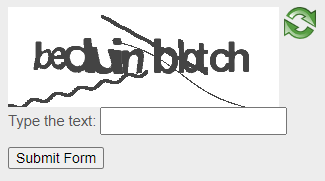
\includegraphics[width=6cm]{gfx/mygraphics/schwierig4.png}
    \caption{Textbasierter CAPTCHA aus der Securimage phpCaptcha Demo, welcher nicht eindeutig zu beantworten ist}
    \label{fig:schwierig}
\end{figure}

Damit würde der CAPTCHA nicht korrekt beantwortet werden können.
Diese Arten der textbasierten CAPTCHAs können gegebenenfalls nicht eindeutig beantwortet werden.
Aus diesem Grund kann bei der Bedienfreundlichkeit keine volle Punktzahl gegeben werden,
sondern es müssen je nach Komplexität ein bis zwei Punkte abgezogen werden.

Zeitliche Begrenzungen können vorkommen, sind aber nicht bei jeder Technik anzutreffen.
Hier ist, sofern gegeben, ebenfalls ein Punkt abzuziehen.

Accessability ist ambivalent zu betrachten.
Textbasierte CAPTCHA allein sind für sehbehinderte Menschen nicht nutzbar. 
Da dies eine Personengruppe vollständig ausschließt, werden zwei Punkte abgezogen.

Ebenso können die verschiedenen Techniken, die bei textbasierten CAPTCHAs angewandt werden, zu Problemen für Legastheniker führen.
Auch Menschen mit Farbfehlsichtigkeiten können durch eine Kombination von ungünstig generierten Hintergründen und Schriftfarben irritiert werden.
Aus diesem Grund wird auch hier jeweils ein Punkt abgezogen.

Einige textbasierte CAPTCHAs lassen sich gut audiobasiert umsetzen, 
um die Accessibility des CAPTCHAs zu gewährleisten. 
Dies würde somit nicht zu einem Punktabzug führen, wie es gegebenenfalls bei reinen audiobasierten CAPTCHAs (\autoref{ch:bewertung:audio}) der Fall wäre.

Die technische Umsetzbarkeit ist bei verschiedenen betrachteten Techniken zur Erstellung und Nutzung textbasierter CAPTCHAs sehr simpel gehalten.
Die Dokumentation ist gut und kann über Programmierschnittstellen (APIs) leicht eingebunden werden. (Vgl. \cite{hcaptcha} \cite{phpcaptcha} \cite{reallysimplecaptcha})
Aus diesem Grund kann hier die volle Punktzahl vergeben werden.

\citeauthor{surveyofresearch} schreiben in \citetitle{surveyofresearch}, 
dass Hollow CAPTCHA durch eine Kombination von Segmentierung und Recognition %TODO
mit einer Erfolgsrate von 36 bis 89 Prozent durch Bots gelöst werden konnten. (Vgl. \cite[p.76ff]{surveyofresearch}) %TODO

Ähnlich verhält es sich bei Überlappungen und CCT (``crowing characters together''):
Hier konnte bei verschiedenen Technologien mithilfe von unterschiedlichen Methoden
eine Erfolgsquote von 27,1 bis 53,2 Prozent erreicht werden. \cite[p.76]{surveyofresearch} %Quellen aus Text noch mit aufnehmen

Auch bei ``noise backgrounds'' und ``two-layer structures'' konnten solche Ergebnisse erzielt werden. 
(Vgl. \cite[p.76]{surveyofresearch})

Auf Basis dieser Erkenntnisse werden textbasierte CAPTCHAs wie in Tabelle \ref{table:matrix:text} bewertet.

%Multifonts, Rotation, Waving, Large character set \cite{surveyofresearch}

\begin{table}[h!]
    \caption{Bewertungsmatrix für textbasierte CAPTCHAs}
    \begin{center}
        \begin{tabular}{l|c}
            Kategorie                       & Bewertung \\\hline
            Bedienfreundlichkeit            & 7-9         \\
            Accessibility                   & 6        \\
            Technische Umsetzbarkeit        & 10         \\
            Sicherheit                      & 3-5         
        \end{tabular}
    \end{center}
    \label{table:matrix:text}
\end{table}

\section{Bildbasierte CAPTCHA}
Bildbasierte CAPTCHAs benötigen etwas mehr Aufwand als beispielsweise textbasierte CAPTCHAs.
Je nach verwendeter Technik muss auf eine Reihenfolge geachtet werden. 
Es ist auch möglich, dass bei einigen Bildern genau darauf geachtet werden muss, ob die gegebenen Antworten wirklich korrekt sind.
In \autoref{fig:fortnite} ist beispielsweise nur schwer zu erkennen, ob manche Hunde wirklich geschlossene Augen haben, 
oder ob der Kontrast zwischen Fell und Iris lediglich zu gering ist.

\begin{figure}[h!]
    \centering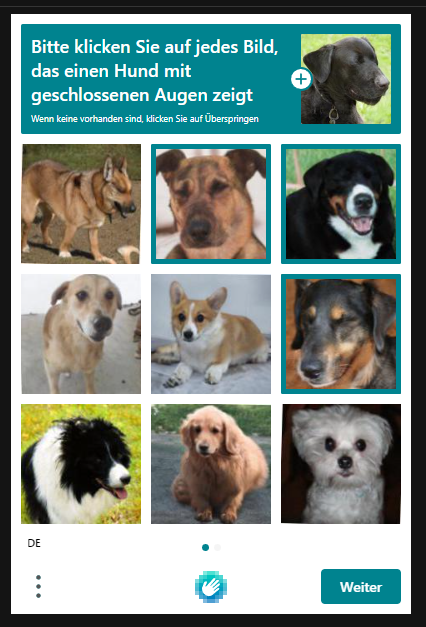
\includegraphics[width=6cm]{gfx/mygraphics/fuerfortnite.png}
 \caption{Bildbasierter CAPTCHA von hCaptcha bei Login auf der Epic Games Website}
      \label{fig:fortnite}
\end{figure}

Bei sehr detailreichen Bildern kann es vorkommen, dass auch ein Mensch mehrere Versuche benötigt, da eventuell nicht jedes gesuchte Objekt sofort erkannt wird.
Deshalb werden bei sehr hoher Komplexität oder bei schwer zu erkennenden Bildern zwischen 2 und 4 Punkte abgezogen werden.
Bei bildbasierten CAPTCHAs kommen zeitliche Begrenzungen eher selten vor. 

Auch hier besteht die Problematik, dass Menschen mit eingeschränker Sicht keine Chance haben, diese Art von CAPTCHAs adäquat auszufüllen.
Es gibt keine Möglichkeit, eine audiobasierte Alternative anzubieten. Durch diese schwerwiegende Einschränkung werden 5 Punkte abgezogen.
Doch auch für Menschen ohne Behinderung kann es, wie bereits erwähnt, schwierig sein, sie erfolgreich zu absolvieren.
Hier verschwimmen die Grenzen bei der Einschätzung des Aufwands und der Accessibility.

Die technische Umsetzbarkeit erfolgt bei bildbasierten CAPTCHAs ebenfalls über APIs. (Vgl. \cite{hcaptcha} \cite{arkoselabs} \cite{geetest})
Analog zu textbasierten CAPTCHAs kann deshalb volle Punktzahl vergeben werden.

Mithilfe einer Support Vector Machine konnte die CAPTCHA-Methode Asirra von Microsoft (Vgl. \cite{elson2007asirra})
mit einer Erfolgsrate von 82,7 Prozent absolviert werden. 
Die Nutzung von OpenCV ermöglicht, bestimmte Merkmale in Bildern algorithmisch zu analysieren.
Ebenso kann durch Trainieren von künstlichen Intelligenzen (KI) durch große Datenmengen (Deep Learning) eine hohe Erfolgsquote erreicht werden,
so konnten bereits mehrere CAPTCHAs von hochrangigen Unternehmen durch diese Weise erfolgreich erledigt durchgeführt werden.
Die Nutzung von KI ist noch nicht allzu weit verbreitet, gewinnt aber immer mehr an Bedeutung.
Da es bereits vermehrt sehr hohe Erfolgsquoten bei der Absolvierung von CAPTCHAs durch KIs und die Nutzung von OpenCV gab,
müssen für beide Techniken zur Umgehung dieser CAPTCHAs 2 Punkte abgezogen werden.
CAPTCHAs, welche über das Verschieben von Reglern funktionieren, sind durch ihr teilweise sehr aufwändiges Tracking von Mausbewegungen,
Reaktionszeit und anderen Metadaten etwas sicherer als selection-based CAPTCHAs. \cite[p.77f]{surveyofresearch}


\begin{table}[h!]
    \caption{Bewertungsmatrix für bildbasierte CAPTCHAs}
    \begin{center}
        \begin{tabular}{l|c}
            Kategorie                       & Bewertung \\\hline
            Bedienfreundlichkeit            & 6-10         \\
            Accessibility                   & 5        \\
            Technische Umsetzbarkeit        & 10         \\
            Sicherheit                      & 6         
        \end{tabular}
    \end{center}
\end{table}

\section{Videobasierte CAPTCHA}
Das Anschauen des jeweiligen Videos nimmt einige Sekunden in Anspruch und man muss dies je nach Komplexität wiederholen, 
da man eventuell nicht alle Aspekte bei dem ersten Durchlauf mitbekommt.
Wie ein Video als CAPTCHA auf Nutzer*innen wirken kann ist nicht genau festzulegen.
Einerseits handelt es sich dabei um etwas aufregenderes als einen simplen Text, andererseits kann dies auch schnell frustrieren.

Videobasierte CAPTCHAs brauchen eine schnelle Internetverbindung, um abgespielt werden zu können. %definiere gut
Desweiteren ist es nicht für jede Nutzer*in möglich zu erkennen, was genau im Video vor sich geht.
Dies führt dazu, dass videobasierte CAPTCHAs eine geringere Accessibility haben als dies bei anderen CAPTCHAs der Fall ist. 

Videobasierte CAPTCHA sind vergleichsweise wenig verbreitet. 
Ein bekannter Anbieter ist die Firma NuData Security mit NuCaptcha.
Nachdem \citeauthor{elie} in ihrem Blogartikel \citetitle{elie} darüber berichtete, 
dass NuCaptcha mit einer 90 prozentigen Erfolgsrate von einem Bot absolviert werden konnte,
wurden zwar einige Änderungen an NuCaptcha vorgenommen, jedoch existiert zum heutigen Tage keinerlei Dokumentation oder ähnliches für NuCaptcha.

Im Jahre 2015 gab es Verfahren, mit denen ein videobasiertes reCAPTCHA mit 31,75 prozentiger Erfolgsrate gebrochen werden konnte. 
Auch hier wirkt sich die Entwicklung besserer Bilderkennungstools und das Trainieren von KI negativ auf die Sicherheit aus.\cite[p.xx]{surveyofresearch}

Da videobasierte CAPTCHAs in der heutigen Zeit kaum noch von Bedeutung sind, werden diese nicht weiter betrachtet.
%\begin{table}[h!]
%    \caption{Bewertungsmatrix für videobasierte CAPTCHA}
%    \begin{center}
%        \begin{tabular}{l|c}
%            Kategorie                       & Bewertung \\\hline
%            Bedienfreundlichkeit            & 6         \\
%            Accessibility                   & 3        \\
%            Technische Umsetzbarkeit        & 2         \\
%            Sicherheit                      & 4         
%        \end{tabular}
%    \end{center}
%\end{table}

\section{Audiobasierte CAPTCHA}
\label{ch:bewertung:audio}

“Buster” ist ein Browser Addon, das reCAPTCHA audio challenges per speech recognition löst.
%
%A. Audio-based CAPTCHA
%This CAPTCHA is usually considered an alternative to a
%visual CAPTCHA in the case of visually impaired users [44].
%Users in most audio-based CAPTCHAs play the role of
%listeners, and they are required to complete the specified
%challenge based on what they have heard. A spoken
%CAPTCHA system was introduced in [45]. This system
%converts a selected word into speech using a Text-To-Speech
%(TTS) system, then plays the sound clip to users and asks them
%to say the word. In 2012, the SoundsRight audio CAPTCHA
%(Fig. 6(a)) provided in [48] asks users to identify a specific
%sound, such as the sound of a bell or a piano. This work has
%increased the success rates in audio Captchas from less than
%50% to over 90% for blind users. Meutzner et al. presented a
%new type of audio CAPTCHA [50] that uses additional
%nonsense speech sounds that are confusing for speech
%recognizers, while being less critical for human listeners. In
%2016, they also proposed a nonspeech audio CAPTCHA [61],
%which is entirely based on the classification of sound events
%mixed into an environmental scene. Moreover, the HuMan
%CAPTCHA designed in [60] asks users to answer the
%presented questions by combining ambient noise and common
%sense knowledge. There is another type of audio-based
%CAPTCHA in which users play the role of speakers and are
%required to pronounce rather than simply listen. For instance,
%Gao et al. [47] proposed a new sound-based CAPTCHA (Fig.
%6(b)) that exploits the differences between a human voice a
%synthetic voice. A user is required to read out a given sentence
%rather than listening an audio file.
%Fig. 6. Examples of audio-based CAPTCHAs
%Attack and defense always go together. A two-stage attack
%for the listener model can always obtain a good attack result.
%In detail, the audio-based CAPTCHA is segmented into
%several regions regarding the location of each spoken word
%first. Then, the regions are recognized by automatic speech
%recognition programs. Tam et al. achieved success rates of up
%to 71% (Google Audio CAPTCHA, reCAPTCHA Audio
%CAPTCHA, Digg CAPTCHA)[44]. Bursztein et al. achieved
%success rates of 45%, 49% and 83% on the CAPTCHAs of
%Yahoo, Microsoft and eBay, respectively[49]. Some
%78
%Authorized licensed use limited to: Fachhochschule FH Darmstadt. Downloaded on July 29,2022 at 08:34:41 UTC from IEEE Xplore. Restrictions apply.
%researchers have even proposed that most of the digit-based
%audio CAPTCHAs are successfully broken with success rates
%between 50%-90% [44][52][54].


\begin{table}[h!]
    \caption{Beispielhafte Bewertungsmatrix}
    \begin{center}
        \begin{tabular}{l|c}
            Kategorie                       & Bewertung \\\hline
            Bedienfreundlichkeit                         & 7         \\
            Accessibility                   & 10        \\
            Technische Umsetzbarkeit        & 3         \\
            Sicherheit                      & 9         
        \end{tabular}
    \end{center}
\end{table}

\begin{table}[h!]
    \caption{Beispielhafte Bewertungsmatrix}
    \begin{center}
        \begin{tabular}{l|c}
            Kategorie                       & Bewertung \\\hline
            Bedienfreundlichkeit                         & 7         \\
            Accessibility                   & 10        \\
            Technische Umsetzbarkeit        & 3         \\
            Sicherheit                      & 9         
        \end{tabular}
    \end{center}
\end{table}

\section{Gamification}

\begin{table}[h!]
    \caption{Beispielhafte Bewertungsmatrix}
    \begin{center}
        \begin{tabular}{l|c}
            Kategorie                       & Bewertung \\\hline
            Bedienfreundlichkeit                         & 7         \\
            Accessibility                   & 10        \\
            Technische Umsetzbarkeit        & 3         \\
            Sicherheit                      & 9         
        \end{tabular}
    \end{center}
\end{table}

\section{Alternativen zu CAPTCHA}

\subsection{Honeypot}

\begin{table}[h!]
    \caption{Beispielhafte Bewertungsmatrix}
    \begin{center}
        \begin{tabular}{l|c}
            Kategorie                       & Bewertung \\\hline
            Bedienfreundlichkeit                         & 7         \\
            Accessibility                   & 10        \\
            Technische Umsetzbarkeit        & 3         \\
            Sicherheit                      & 9         
        \end{tabular}
    \end{center}
\end{table}

\subsection{Anti Spam Plugins}

\begin{table}[h!]
    \caption{Beispielhafte Bewertungsmatrix}
    \begin{center}
        \begin{tabular}{l|c}
            Kategorie                       & Bewertung \\\hline
            Bedienfreundlichkeit                         & 7         \\
            Accessibility                   & 10        \\
            Technische Umsetzbarkeit        & 3         \\
            Sicherheit                      & 9         
        \end{tabular}
    \end{center}
\end{table}

\subsection{Multi-Faktor Authentifikation}

\begin{table}[h!]
    \caption{Beispielhafte Bewertungsmatrix}
    \begin{center}
        \begin{tabular}{l|c}
            Kategorie                       & Bewertung \\\hline
            Bedienfreundlichkeit                         & 7         \\
            Accessibility                   & 10        \\
            Technische Umsetzbarkeit        & 3         \\
            Sicherheit                      & 9         
        \end{tabular}
    \end{center}
\end{table}

\subsection{Biometrie}

\begin{table}[h!]
    \caption{Beispielhafte Bewertungsmatrix}
    \begin{center}
        \begin{tabular}{l|c}
            Kategorie                       & Bewertung \\\hline
            Bedienfreundlichkeit                         & 7         \\
            Accessibility                   & 10        \\
            Technische Umsetzbarkeit        & 3         \\
            Sicherheit                      & 9         
        \end{tabular}
    \end{center}
\end{table}